\documentclass[xetex,aspectratio=43]{beamer}

\usepackage{res/lections}

\preamble

\title{Устройства хранения данных}

\begin{document}

    \titleslide

    \tocslide


\section{Контроль ошибок (на экзамен не выносится)}

\begin{frame}{Коды обнаружения}
\defn{Код обнаружения (контрольная сумма)}{ избыточные данные, которые позволяют \emph{не достоверно} контролировать корректность основных}

Вычислительные:

\begin{itemize}
\tightlist
\item
  Сумма всех битов по модулю 2
\item
  CRC и другие легко аппаратно реализуемые контрольные суммы
\end{itemize}

Из «повседневной жизни»:

\begin{itemize}
\tightlist
\item
  Последние символы в ISSN и номерах банковских карт
\end{itemize}
\end{frame}

\begin{frame}{Коды коррекции}
\defn{Код коррекции}{избыточные данные,
которые позволяют \emph{не достоверно} обнаруживать и исправлять ошибки в
основных}

\begin{itemize}
\tightlist
\item
  Обнаруживают ошибки в \(N\) битах
\item
  Исправляют в \(M\le N\) битах
\end{itemize}

Пример --- \href{http://en.wikipedia.org/wiki/Hamming_code}{код
Хэмминга}, обнаруживает не более 2 и исправляет не более 1 ошибки.
\end{frame}

\begin{frame}{Код Хемминга для исправления 1 ошибки: теория}
\(D_0 = \{2^n | n \in [1,16)\}\),\(f_0 (x) = \log_2 x\),
\(f_0:D_0 \leftrightarrow R_0,\)\\
\(R_0 = \{f_0(x) | x \in D_0\}\)

\pause

Вводятся бинарные (групповые) операции \(\bigoplus_D, \bigoplus_R\)

\begin{enumerate}
\item
  \(D\) --- замыкание \(D_0\) относительно \(\bigoplus_D\)
\item
  \(f : D \rightarrow R (R=R_0), f(x) = f_0(x) \forall x \in D_0\) ---
  расширение \(f_0\)
\item
  \(f\) строится, как гомоморфизм:
  \(f(x_1\bigoplus_D x_2) = f(x_1)\bigoplus_R f(x_2)\)
\end{enumerate}
\end{frame}

\begin{frame}{Код Хемминга для исправления 1 ошибки: пример}
Отправили: \(x_1; f(x_1)\)\\
Пришло: \(x'\_1 = x\_1 \bigoplus x', x' \in D\_0; f\_{x\_1} = f(x\_1)\),
причём \(x'\) мы не знаем.

Тогда
\(s = f_{x_1} \bigoplus f(x'_1) = f(x_1) \bigoplus f(x_1) \bigoplus f (x') = f(x').\)\\
Но \(x' = f^{-1}(s)\) --- нашли ошибочный бит.
\end{frame}

\begin{frame}{Код Хемминга для обнаружения 2 ошибок}
Практика Послали: \(x_1; f(x_1)\)\\
Пришло:
\(x'\_1 = x\_1 \bigoplus x'\_a \bigoplus x'\_b, x'\_a, x'\_b \in D\_0; f\_{x\_1} = f(x\_1)\),
причём \(x'_a, x'_b\) мы не знаем.

Но \(\forall x'_a \not = x'_b\) справедливо
\(f(x'_a \bigoplus x'_b) \not = 0\),\\
а значит \(f(x_1 \bigoplus x'_a \bigoplus x'_b) \neq f(x_1)\),\\
т.е. ошибка будет обнаружена, хотя сами \(x'_a, x'_b\) мы так и не
узнаем.

\pause

Важно: Мы не сможем узнать, была ли ошибка одна и она была успешно
исправлена, или же их было две (или даже больше), и они были исправлены
неправильно.

Если ошибок было больше двух, мы вообще можем о них не узнать.

\end{frame}

\section{Энергонезависимая память}

\begin{frame}{Краткая история}
    \begin{figure}
        
\includegraphics[height=0.8\textheight]{img/\jobname/evo.jpg}
    \end{figure}
\end{frame}

\subsection{Природа носителя данных}

\begin{frame}{Бумага}

\begin{itemize}
\tightlist
\item
  Конспект
\item
  Перфокарта
\item
  Перфолента

\end{itemize}
\end{frame}

\begin{frame}{Магнитные устройства}

\begin{itemize}
\tightlist
\item
  Лента

  \begin{itemize}
  \tightlist
  \item
    Долго мотать до оглавления
  \item
    Ломается, крошится магнитный слой
  \item
    Высокая скорость
  \end{itemize}
\item
  Барабан

  \begin{itemize}
  \tightlist
  \item
    Весьма быстрый (на некоторых ЭВМ использовался, как ОЗУ)
  \item
    Громоздкий, сейчас не используется
  \end{itemize}
\item
  Диски
\end{itemize}
\end{frame}

\subsection{Диски: жёсткие и не очень}

\begin{frame}{Магнитные устройства: Диски дискеты и прочие друзья (I)}
\begin{itemize}
\tightlist
\item
  Сменные быстрые пакеты

  \begin{itemize}
  \tightlist
  \item
    Пришли на смену барабанам
  \item
    \href{http://www.ixbt.com/storage/hdd50years.shtml}{Экранолетные
    головки}
  \end{itemize}
\item
  ГМД

  \begin{itemize}
  \tightlist
  \item
    Почти 40 лет (1971 -- 2010(?))
  \item
    От 80 килобайт (и 8 дюймов) до 2.88 МиБ (3.5 дюйма)
  \end{itemize}
\item
  Сменные магнитно-оптические носители

  \begin{itemize}
  \tightlist
  \item
    Нагрев до точки Кюри + размазанное магнитное поле. По 100 МиБ Лазер
    легко сфокусировать
  \end{itemize}
\end{itemize}
\end{frame}

\begin{frame}{Магнитные устройства: Жёсткие диски (I)}

\begin{itemize}
\item
  \href{https://en.wikipedia.org/wiki/Hard_disk_drive\#Components}{Компоненты}
\item Перемещение коромысла «непрерывное»
\item
  \href{https://commons.wikimedia.org/w/index.php?title=File\%3AHardDisk1.ogv}{Вид
  изнутри}
\item
  Типично использование
  \href{https://ru.wikipedia.org/wiki/\%D0\%93\%D0\%B8\%D0\%B4\%D1\%80\%D0\%B0\%D0\%B2\%D0\%BB\%D0\%B8\%D1\%87\%D0\%B5\%D1\%81\%D0\%BA\%D0\%B8\%D0\%B5_\%D0\%B8_\%D0\%BF\%D0\%BD\%D0\%B5\%D0\%B2\%D0\%BC\%D0\%B0\%D1\%82\%D0\%B8\%D1\%87\%D0\%B5\%D1\%81\%D0\%BA\%D0\%B8\%D0\%B5_\%D0\%BF\%D0\%BE\%D0\%B4\%D1\%88\%D0\%B8\%D0\%BF\%D0\%BD\%D0\%B8\%D0\%BA\%D0\%B8}{гидродинамических подшипников}
\end{itemize}

\pause

А ещё при помощи жёсткого диска, как и почти любого механического
устройства, \href{https://youtu.be/pmfHHLfbjNQ}{можно воспроизводить
звук}
\end{frame}

\begin{frame}{Магнитные устройства:  Жёсткие диски (II)}

\begin{outline}
    \tightlist
    \1 Жесткий --- твердый и несменный
    \1 Быстрые, высокая плотность
    \1 Многократная перезапись, обычно экранолетные головки
    \1 Пример сменных --- ZIPdrive --- не слишком удачный
    \1 История:
        \2 Первый --- \href{https://en.wikipedia.org/wiki/IBM_305_RAMAC}{IBM 350 RAMAC}, 1956 г., 1 тонна, 5 мегабайт --- для мейнфреймов и табуляторов
        \2 1980 --- 5,25 Winchester, Shugart ST-506, 5 МиБ
        \2 2006 --- гибридные --- диск + несколько ГиБ Flash --- во Flash --- КЭШ write-back, мотор стоит, ноутбук работает дольше. Промышленный образец --- Seagate Momentus XT --- 2010/
        \2 Вектор записи
            \3 2006 --- перпендикулярная запись
            \3 2013 --- «\href{https://en.wikipedia.org/wiki/Shingled\_magnetic\_recording}{черепичная запись}» --- для изменения приходится перезаписать сектора нескольких дорожек
\end{outline}
\end{frame}

\subsection{Оптические носители}

\begin{frame}{Оптические носители}
\begin{itemize}
\tightlist
\item
  CD
\item
  DVD
\item
  Blue Ray / HD DVD
\end{itemize}
\end{frame}

\begin{frame}{CD}
        \begin{itemize}
            \tightlist
            \item
            1979 год
            \item
            Дорожка по спирали
            \item
            Единица скорости --- около 150 КиБ/сек
            \item
            Впадины по 0,8 микрона
            \item
            Постоянная линейная скорость
        \end{itemize}

        RW --- пузырьками в пластике
\end{frame}

\begin{frame}{DVD}
        \begin{itemize}
            \tightlist
            \item
            Единица скорости --- около 1350 КиБ/сек
            \item
            Впадины по 0,4 микрона (частота луча, больше, теорема Котельникова)
            \item
            Многослойные
            \item
            Коды регионов
        \end{itemize}
\end{frame}

\begin{frame}{ВluRay и HD DVD}
        \begin{itemize}
            \tightlist
            \item
            Blu

            \begin{itemize}
                \tightlist
                \item
                Четырехслойные до 100 ГиБ
            \end{itemize}
            \item
            HD

            \begin{itemize}
                \tightlist
                \item
                Трехслойные до 45 ГиБ
            \end{itemize}
        \end{itemize}

\end{frame}

\begin{frame}{Долговечность}
    \begin{block}{Ширпотреб}
        \begin{outline}
            \1 Самые долговечные --- заводские
            \1 Самые недолговечные --- RW
            \1 Долговечность CD/DVD R
                \2 CD-R и DVD-R --- 10--25 лет, органический носитель данных
                \2 BD-R --- 25--50 лет, металлический носитель данных
        \end{outline}
    \end{block}
    \pause
    А если хочется подольше?
    \pause
    \begin{block}{M-DISC}
        Полностью --- \href{https://ru.wikipedia.org/wiki/M-DISC}{Millennial Disc}
        \begin{itemize}
            \item DVD- и BD-R
            \item Слой с данными специального состава, обещают сотни лет
            \item Требует более мощного лазера для записи
        \end{itemize}
        Тоже почти ширпотреб: болванки дороже раз в пять, привод --- раза в 2--3
    \end{block}
\end{frame}

\subsection{Твердотельные накопители}

\begin{frame}{Твердотельные накопители (Solid State Drives)}
    Твердотельные --- накопители без движущихся механических деталей

    \begin{itemize}
        \tightlist
        \item
        «Исключительно высокая» скорость позиционирования (позиционирования,
        как такового, нет)
        \item
        Достаточно высокая скорость записи
        \item
        Высокая скорость чтения
    \end{itemize}

    \pause

    \begin{itemize}
        \tightlist
        \item
        Не боятся перегрузок
        \item
        Имеют конечный ресурс из-за свойств элементов памяти
        \item
        Удельная цена за бит выше, чем у механических
    \end{itemize}

\end{frame}

\begin{frame}
    \begin{block}{Flash-память}
        Самый распространённый и дешёвый вид --- NAND. Построена на транзисторах
        с плавающими затворами, низкий ресурс, десятки тысяч переключений

        \begin{itemize}
            \tightlist
            \item
            Старые флешки можно было за несколько часов испортить, если записывать
            в одну и ту же область
            \item
            Довольно быстро флешки стали умнее и научились переназначать области:
            если в какую-то область часто записывали, контроллер менял её местами
            с другой, менее «популярной»
        \end{itemize}
    \end{block}
\end{frame}

\begin{frame}[fragile]
    \begin{block}{Твердотельный накопитель}
        \begin{itemize}
            \tightlist
            \item
            Фактически --- параллельно несколько из флешек, что обеспечивает высокие скорость и
            ёмкость
            \item
            Подключается через SATA или PCI Express
        \end{itemize}

        Для ускорения переноса «популярных» областей в протоколе SATA есть
        команда \texttt{IDLE}. Накопитель не знает формата файловой системы и не
        в курсе, занята область, или свободна, но ОС может подсказать, что
        обасть свободна. Тогда накопитель при переносе данных в эту область не
        будет переносить данные из неё ещё куда-то, что хорошо для скорости и
        ресурса.

    \end{block}
\end{frame}

\begin{frame}[fragile]{Энергонезависимость основной памяти}

    Проф. В.М. Нестеров (тогда директор СПб отделения EMC, профессор в
    СПбГУ), конференция СПИСОК-2016:

    \begin{quote}
        \href{http://spisok.math.spbu.ru/video/2016/4.mp4}{К 2020 г. ожидается стирание грани между твердотельной энергонезависимой памятью и оперативной памятью в плане производительности и цены}, время: 42:50
    \end{quote}

    \pause

    Высказывались и более сильные предположения, например, что скоро вся память будет энергонезависимой

    \begin{itemize}
        \tightlist
        \item
        Успехи твердотельных накопителей на рынке впечатляют, но пока до этого далеко
        \item
        Тем не менее в перспективе это реально

        \begin{itemize}
            \tightlist
            \item
            Серьёзный вызов архитекторам ПО и ЭВМ --- это многое может изменить
        \end{itemize}
    \end{itemize}

\end{frame}

\section{Redundant Array of Inexpensive Disks}


\begin{frame}{RAID 0}
    \begin{figure}
        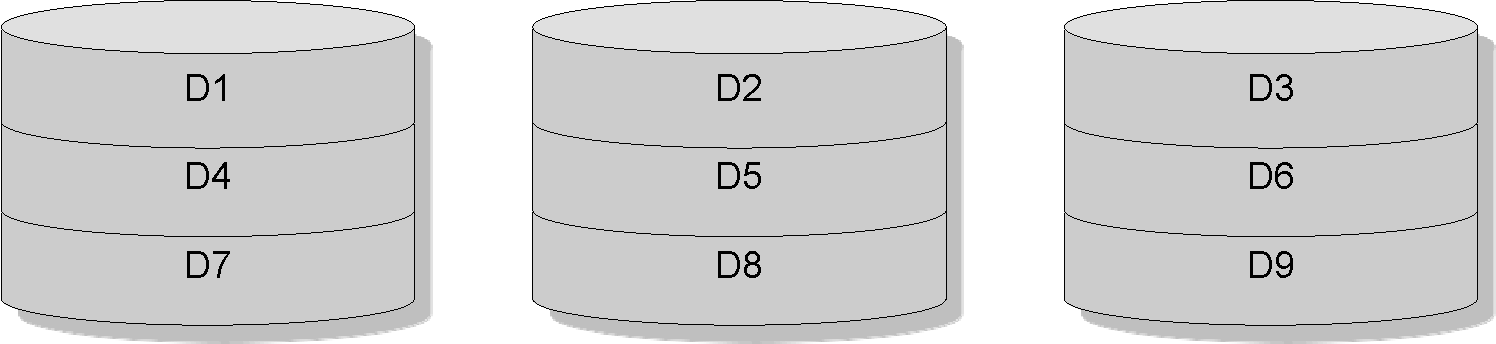
\includegraphics[width=0.75\textwidth, page=1]{img/\jobname/raids-crop.pdf}
    \end{figure}

\begin{itemize}
\tightlist
\item
  \(N\) устройств
\item
  Сектора адресуются последовательно на разных винчестерах
\item
  Избыточности нет
\item
  Скорость чтения/записи и емкость растут в N раз
\item
  Надежность падает
\end{itemize}
\end{frame}

\begin{frame}{RAID 1}
    \begin{figure}
        \includegraphics[width=0.75\textwidth, page=2]{img/\jobname/raids-crop.pdf}
    \end{figure}

\begin{itemize}
\tightlist
\item
  \(M\) устройств
\item
  «Зеркальные» диски
\item
  Есть избыточность
\item
  Надежность растет
\item
  Скорость чтения растет в M раз, скорость записи старая
\end{itemize}
\end{frame}

\begin{frame}
\begin{block}{RAID 0+1}
\begin{itemize}
\tightlist
\item
  \(N\times M\) устройств
\item
  Комбинирует 0 и 1 (0 поверх 1 или 1 поверх 0 --- «коммутируют»)
\item
  Надежность в целом растет
\item
  Скорость чтения растет в \(N\times M\) раз, записи --- в N раз,
  емкость в N
\item
  Избыточность есть
\end{itemize}
\end{block}
\end{frame}

\begin{frame}{RAID 2, 3 и 4}
    \begin{figure}
        \includegraphics[width=0.75\textwidth, page=3]{img/\jobname/raids-crop.pdf}
    \end{figure}

\begin{itemize}
\tightlist
\item
  2 --- Данные разбиваются по битам (8 накопителей) + еще несколько на
  коды восстановления
\item
  3, 4 --- Примерно как RAID 2, только блоки больше
\item
  Недостаток: высокая нагрузка на диски с кодами восстановления
\end{itemize}
\end{frame}

\begin{frame}{RAID 5}
    \begin{figure}
        \includegraphics[width=0.75\textwidth, page=4]{img/\jobname/raids-crop.pdf}
    \end{figure}

\begin{itemize}
\tightlist
\item
  Коды восстановления информация поочередно появляется на разных дисках
\item
  При выходе из строя одного диска сильно нагружается ---
  восстанавливаются данные
\end{itemize}

А что там за коды восстановления?

\pause

Элементарно!

\[S(i..j) = \displaystyle\bigoplus_{k=i}^jD(k)\]
\end{frame}

\begin{frame}{RAID 6}
    \begin{figure}
        \includegraphics[width=0.75\textwidth, page=5]{img/\jobname/raids-crop.pdf}
    \end{figure}

А что там за коды восстановления?

\pause

Не элементарно: коды Рида-Соломона и всякая довольно задумчивая алгебра\ldots
\end{frame}

\begin{frame}{НищеRAID}
    Вообще RAID можно сделать из чего угодно:
    \begin{itemize}
    \item \href{https://youtu.be/dougISKs2vQ}{Из настоящих флешек}
    \item \href{https://youtu.be/Uxj7So3h-lw}{Из дисководов с дискетами}
    \end{itemize}
\end{frame}

\begin{frame}{Вопросы и упражнения}
\begin{block}{Вопросы}
\begin{itemize}
\tightlist
\item
  Что такое коды обнаружения и коррекции?
\item
  Назовите исторические и современные виды энергонезависимой памяти
\item
  Назовите основные характеристики жёстких дисков
\item
  Перечислите типы и опишите модели размещения данных RAID разных
  уровней
\item
  Какими свойствами в сравнении с механическими жёсткими дисками
  обладают твердотельные накопители?
\item
  Для чего в протоколе SATA есть команда \texttt{IDLE}?
\end{itemize}
\end{block}

\begin{block}{Упражнения}
\begin{itemize}
\tightlist
\item
  Попробуйте произвольно «извлечь» звук из Floppy-дисковода (или из чего-нибудь другого =))

  \begin{itemize}
  \tightlist
  \item
    На «высоком уровне» можно попытаться это сделать, отформатировав
    дискету, записав на неё файл на весь объём, и обращаясь к разным его
    участкам
  \item
    На низком уровне это можно сделать, изучив программный интерфейс
    соответствующего драйвера
  \end{itemize}
\end{itemize}
\end{block}
\end{frame}

\postamble

\end{document}
